% !TeX root = ../thesis_main.tex

% ---------------------------------------------------
% ----- Chapters of the template
% ----- for Bachelor-, Master thesis and class papers
% ---------------------------------------------------
%  Created by C. Müller-Birn on 2012-08-17, CC-BY-SA 3.0.
%  Freie Universität Berlin, Institute of Computer Science, Human Centered Computing. 
%
\chapter{Implementation and deployment}
\label{chap:impl} 

% The phase of implementation and deployment followed an agile development process where changes could be deployed easily to get fast feedback from users.
This chapter describes the agile development process used for implementation of the UI Editor and gives examples on features. The code can be seen at \url{https://git.imp.fu-berlin.de/matthiak00/thesis-ui-builder-snapshot}\footnote{snapshot from Sprylab's Gitlab on 2023-01-25, accessible for members of the \url{https://git.imp.fu-berlin.de} instance}.

% \localtableofcontents

\section{Architecture}

The architecture and high-level user flows of the three software components relevant for the UI editor include the frontend, backend, and \Gls{manager} backend. The Purple Manager backend handles authentication, app management, and providing dynamic resources as ZIP files. The user journey begins with logging in at the root domain (e.g. \url{https://builder.purplemanager.com}, but the details of authentication will not be covered as it is not relevant for the user experience. The \Gls{rest} of the Purple Manager and the dynamic resource management are basic technical requirements set by the surrounding ecosystem.
Fig. \ref{fig:userflow} displays a typical interaction of a user with the editor frontend after selecting an app; pulling the latest dynamic resources, editing a file and merging the changes.
\begin{figure}[h!]
  \centering
  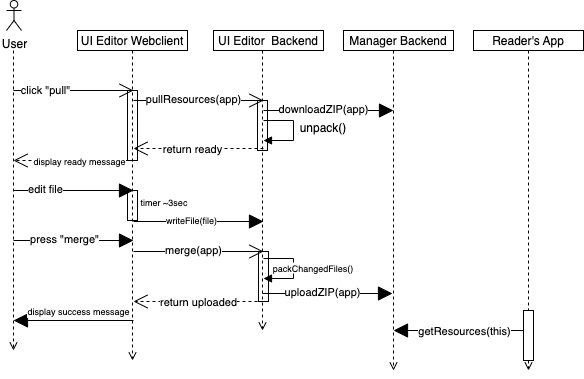
\includegraphics[width=0.9\textwidth]{pics/user-flow.uml.drawio.png}
  \caption{A typical interaction of a user with the UI Editor}
  \label{fig:userflow}
\end{figure}
\pagebreak
\section{Software stack}
From a company's perspective, it is advantageous to keep the software stack as small as possible.
For this case study, the most important point was the availability of additional personnel with knowledge about the frameworks and languages used.
To conform with the company's \Gls{devops} practices the only requirement is to run the project inside Docker containers in a \Gls{kubernetes} environment.
\\\\
For this project the Typescript language (\url{https://www.typescriptlang.org}) is used on back- and frontend.
The advantage is the availability of skilled personnel in the company as well as an established ecosystem and easy sharing of code and type definitions between frontend and backend. The following list gives an overview of the most important tools used:

\begin{description}
  \item[Frontend] \leavevmode
  \begin{description}
    \item[Rendering framework] \textendash{} \textit{React JS v18} (\url{https://reactjs.org/})
    \item[UI Component Library] \textendash{} \textit{Blueprint JS} (\url{https://blueprintjs.com/}) provides components so a consistent design system with common functionality like buttons, dropdowns, filters etc. can be used.
    \item[Other libraries] \textendash{} \textit{ReactQuery / TanQuery} to manage, cache and invalidate HTTP API requests to the backend, \textit{Zustand JS} for shared reactive state management and \textit{Zod} for type validation at runtime.
  \end{description}
  \item[Backend] \leavevmode
  \begin{description}
    \item[HTTP Server] \textendash{} \textit{Express} on \textit{Node JS}, which is the most common combination to run an JavaScript based HTTP server (see \cite{Github:VanoDevium/node-framework-stars}).
    \item[Routing abstraction] \textendash{} \textit{TSOA} (\url{https://github.com/lukeautry/tsoa}) on top of \textit{Express}, which is a Typescript library to provide Java-Spring like syntax with controllers, dependency injection and parameter validation at runtime.
  \end{description}
  \item[Testing] \textendash{} \textit{Vitest} (\url{https://vitest.dev/}) for unit tests and \textit{Playwright} (\url{https://playwright.dev/}) as E2E test runtime. 
  \item[DevOps] \textendash{} \textit{Gitlab Pipelines} to build, test and package on every merge request or commit to develop and master branch.
  \item[Project Setup] \textendash{} Monorepository with \textit{PNPM} as package manager and \textit{Turborepo} to manage package dependencies and automatic optimal build scheduling and caching.
\end{description}

\section{Continuous Integration / Continuous Delivery}

Continuous Integration and Continuous Delivery (CI/CD), a core practice of agile software development, is crucial for agile prototyping and development and enables fast release and deployment cycles.
A Gitlab CI/CD Pipeline was set up for the UI builder, consisting of build, package, and deploy stages.
The build stage also executed unit and end-to-end tests due to technical reasons for efficiency.\\
Having a fast and reliable CI/CD process during development and prototyping was valuable, as it allowed quick response to user feedback and deployment to a staging domain in under 10 minutes.
Separating staging and production systems allowed more confident deployment of quick fixes for validation in a production-like environment without interrupting users.

\section{Feature examples}

A selection of features implemented for the UI Editor is presented in the following section.
These features are examples of how the HCI methods and outcomes from the user research phase influenced their design and how they can improve the user's experience. 

\subsection{File management - multiple file tabs}

A common workflow consists of editing multiple files simultaneously, for example having the view configuration open while adding translations for newly added components.
The old editor tool allowed opening only one file at a time, which got closed automatically when the user opened another file.
During the moderated observation this showed up as a big slowdown.
All participants mentioned that they have to work on multiple files and are annoyed by this workflow.
Especially the opening of large files can take more than 30 seconds.
\\
The solution was inspired by the file management that most \Gls{ide}s provide; a bar on top where all the opened files are listed so the user can quickly switch between them or even close not needed ones (see fig. \ref{fig:file-tabs}). 

\begin{figure}[h!]
  \fbox{
    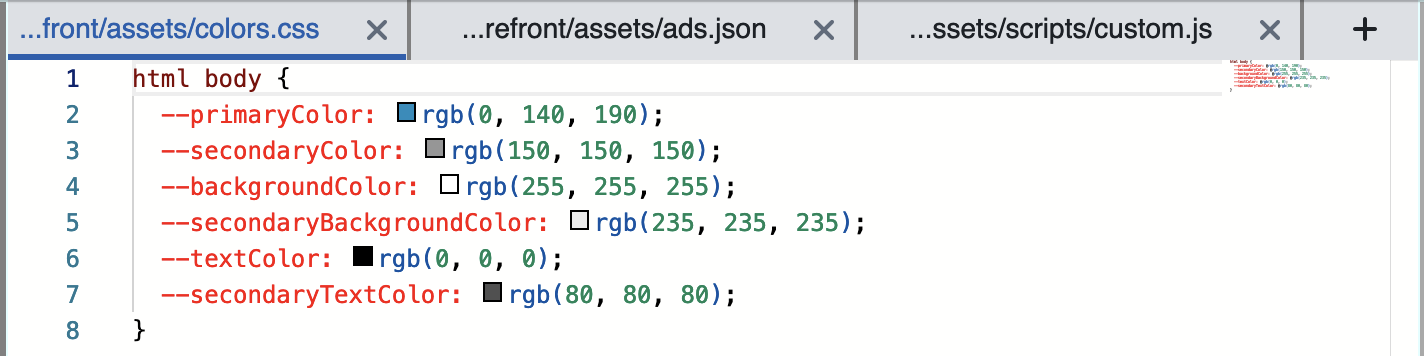
\includegraphics[width=\textwidth]{pics/file_tabs.png}
  }
  \caption{Screenshot of file tabs}
  \label{fig:file-tabs}
\end{figure}

\subsection{File management - quick links}

A second feature regarding the file management is ``quick links''. While all target groups benefit from this, especially for the personas \textit{Steffi, \ref{persona:productdev}} and \textit{Karsten, \ref{persona:itpublishing}}
this can speed up common tasks considerably.

The basic idea is to bookmark frequently used files, e.g. the translation or ad config, and have them prominently available when opening a new app.
For the implementation, three questions needed to be answered:
\begin{description}
  \item[Where to save?] The quick links are stored in the \Gls{localstorage} of the user's browser, so the list is available across apps.
  \item[How to manage?] The user has a list on the settings view, where entries can be added, deleted and changed, but the file path needs to be inserted manually. A screenshot of the settings can be seen in Appendix \ref{fig:settings}. To enhance the user experience, a proposal exists to either add a file picker in the settings or add a bookmark button to the file manager.
  \item[How to present the links?] The links must be easily accessible to provide the intended benefit. The solution was to show them prominently when entering the edit view and no file was opened yet. Based on user feedback, each link shows via an icon whether it links to a folder which the file explorer navigates to (1), to a file which gets opened in a new file tab (2), or if the path does not exist in the current app (3).
  \begin{figure}[h!]
    \centering
    \fbox{
      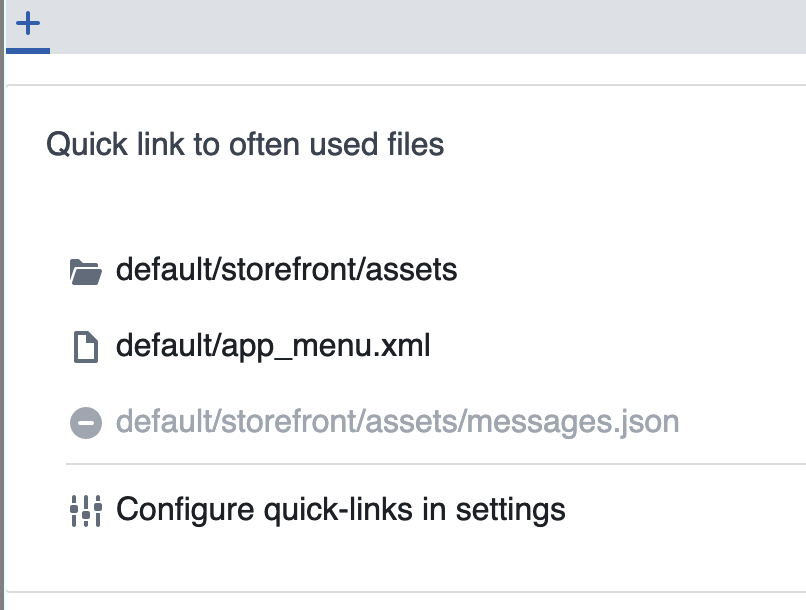
\includegraphics[width=0.5\textwidth]{pics/quick_links.png}
    }
    \caption{The three types of quick links visualized with icons}
  \end{figure}
\end{description}
\subsection{Editor - Abstraction to provide per-file custom editors}

Purple Experience relies on a variety of configuration files, all with different schemata and functional intents.
To provide an efficient and error reduced workflow to users, it is important to have different specialized file editors.

For view configurations for example, the JSON Editor Library (\url{https://github.com/json-editor/json-editor}) is used, combined with the generated JSON Schema files.

For the translations there exists a custom editor that has a fuzzy search function and makes it easy to manage translation entries.

The abstraction is done solely in the frontend and follows React's ``\Gls{comp-over-inh}'' pattern (see fig. \ref{fig:abstract-editor}). Due to modern React JS architecture, component classes are replaced with functional components (marked with $\ll functional\gg$).
To integrate a new specialized editor type, the only two steps are necessary:
Creating a new functional component that implements the \textit{EditorImpl} interface
and adding that editor in the \textit{EditorRegistry} to get returned for the file paths requested.
\begin{figure}[h!]
  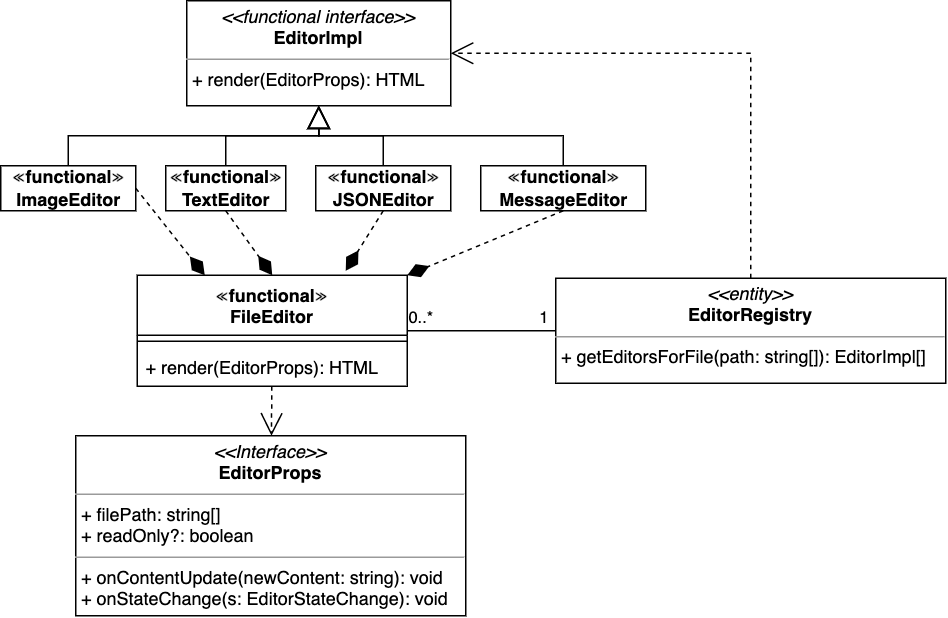
\includegraphics[width=\textwidth]{pics/abstract_editor_uml.drawio.png}
  \caption{Class diagram showing the editor abstraction in React JS.}
  \label{fig:abstract-editor}
\end{figure}
Examples of custom editor implementations can be seen in Appendix \ref{fig:messages_editor} and \ref{fig:ads-editor}.
By implementing Editors for multiple levels of expertise, users like persona ``Karsten'' (\ref{persona:itpublishing}) can make small adaptions like changing a translation without worrying about the underlying file format and without the possibility to break the app due to syntax errors.

\section{Automated Testing}
\label{sec:automated-testing}

Automated tests contribute to the confidence of developers to deploy more frequently and can reduce load from the QA team to test common workflows over and over.
Two of the most common testing levels were used for the project: unit tests and End-to-End tests (also known as E2E or System tests).
\\\\
Unit tests check one ``component'' in a sandboxed environment, often done per-function or per-class.
On the client, both UI components and business logic code that is encapsulated in classes or JavaScript modules get tested.

They also enable Test-driven development, where the tests are written upfront based on specifications and constraints with invariants, pre- and postconditions and the code is continously tested against them.
\\
For agile development, the speed of the test execution and CI/CD Pipelines is important. The developer is blocked during that time and can not progress on the task.
Therefore, the aim was to find a fast runtime, compatible with UI and browser testing as well as Node JS for server code.
After evaluating commonly used test frameworks, Vitest (\url{https://vitest.dev/}) was chosen which fulfills all the requirements. Tests can be hot-reloaded and re-executed on change in less than a second, providing a good developer experience.
\\\\
Due to the complexity of interoperation between components, APIs and the Web standards, unit tests alone are not enough to guarantee the different modules work together as expected. 
\\
E2E tests are supposed to cover a typical user interaction with the service to validate the interaction between business logic components, UI and the user.
First a headless browser\footnote{Headless browsers are browser instances that do not render the actual content to a user's screen, but run as a CLI application and still execute all JavaScript, CSS and HTML.} (\url{https://pptr.dev/}) was used in combination with Vitest,
but writing and debugging tests proved to be slow and error-prone.
\\\\
Later in the process, the E2E tests were rewritten for an alternative test framework called Playwright (\url{https://playwright.dev/}), which allows recording a test case in a normal browser window and then generates the test code automatically, allowing to be adapted and generalized if needed.
After the tests were ported to the new framework, developers can enjoy better debugging tools and the ability to add new tests easier. This may be an example to others that investing time in researching new tools and refactoring code is worthwhile, increasing developer experience and, in turn, speed and confidence.

\section{Privacy-friendly analytics \& monitoring}
\label{sec:analytics}

Sooner or later, you find yourself in a pickle when it comes to tracking.
On the one hand, the data can provide valuable insights into the behavior of many users, which would not be possible through qualitative research.
On the other hand, the most common tools like Google Analytics track users with cookies, which creates new challenges regarding GDPR compliance.
\\\\
The Purple product owner proposed \url{https://squeaky.ai/}, a cookieless solution to track users on this page.
While it can not provide the same level of demographic information a cookie based solution can, it still collects the most important data like usage statistics, user interactions and occurred JavaScript errors.
It can even show heatmaps per page to visualize which UI elements the user interacts with the most.

These heatmaps for example can show whether a new UI feature is used and how users interact with the page in general.
Fig. \ref{fig:squeaky} shows that users mostly interacted with the file explorer and only did a few clicks in the editor panel.
\begin{figure}[h!]
  \centering
  \fbox{
    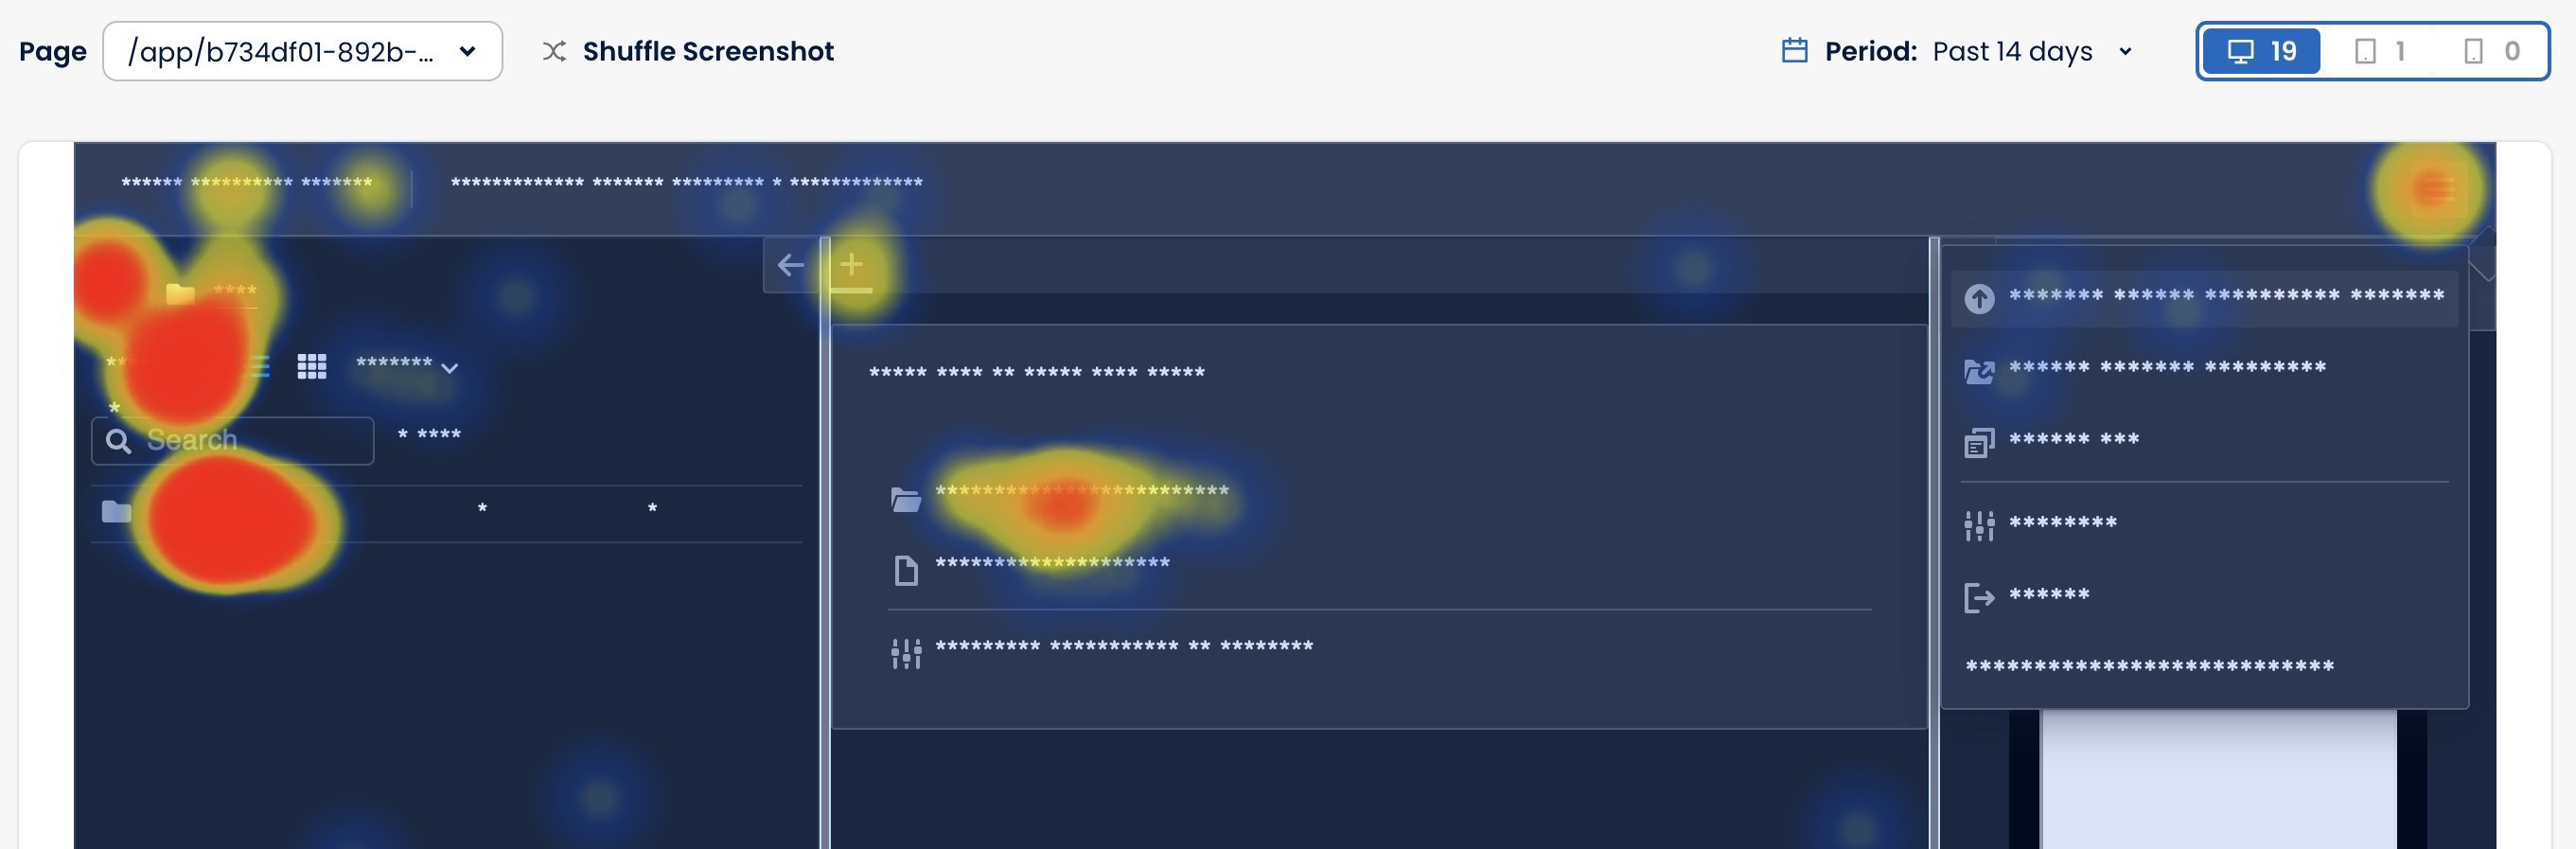
\includegraphics[width=\textwidth]{pics/squeaky_heatmap.jpg}
  }
  \caption{Screenshot: Squeaky.ai heatmap of an app's edit view}
  \label{fig:squeaky}
\end{figure}

To analyze the usage growth, fig. \ref{fig:squeaky_users} indicates how the number of page views per week increased steadily since the internal beta version was launched (except the holiday dip).
The graph clearly shows that the time-bound goal from the SMART criteria in chapter \ref{fig:smart} has been successfully achieved.

\begin{figure}[h]
  \centering
  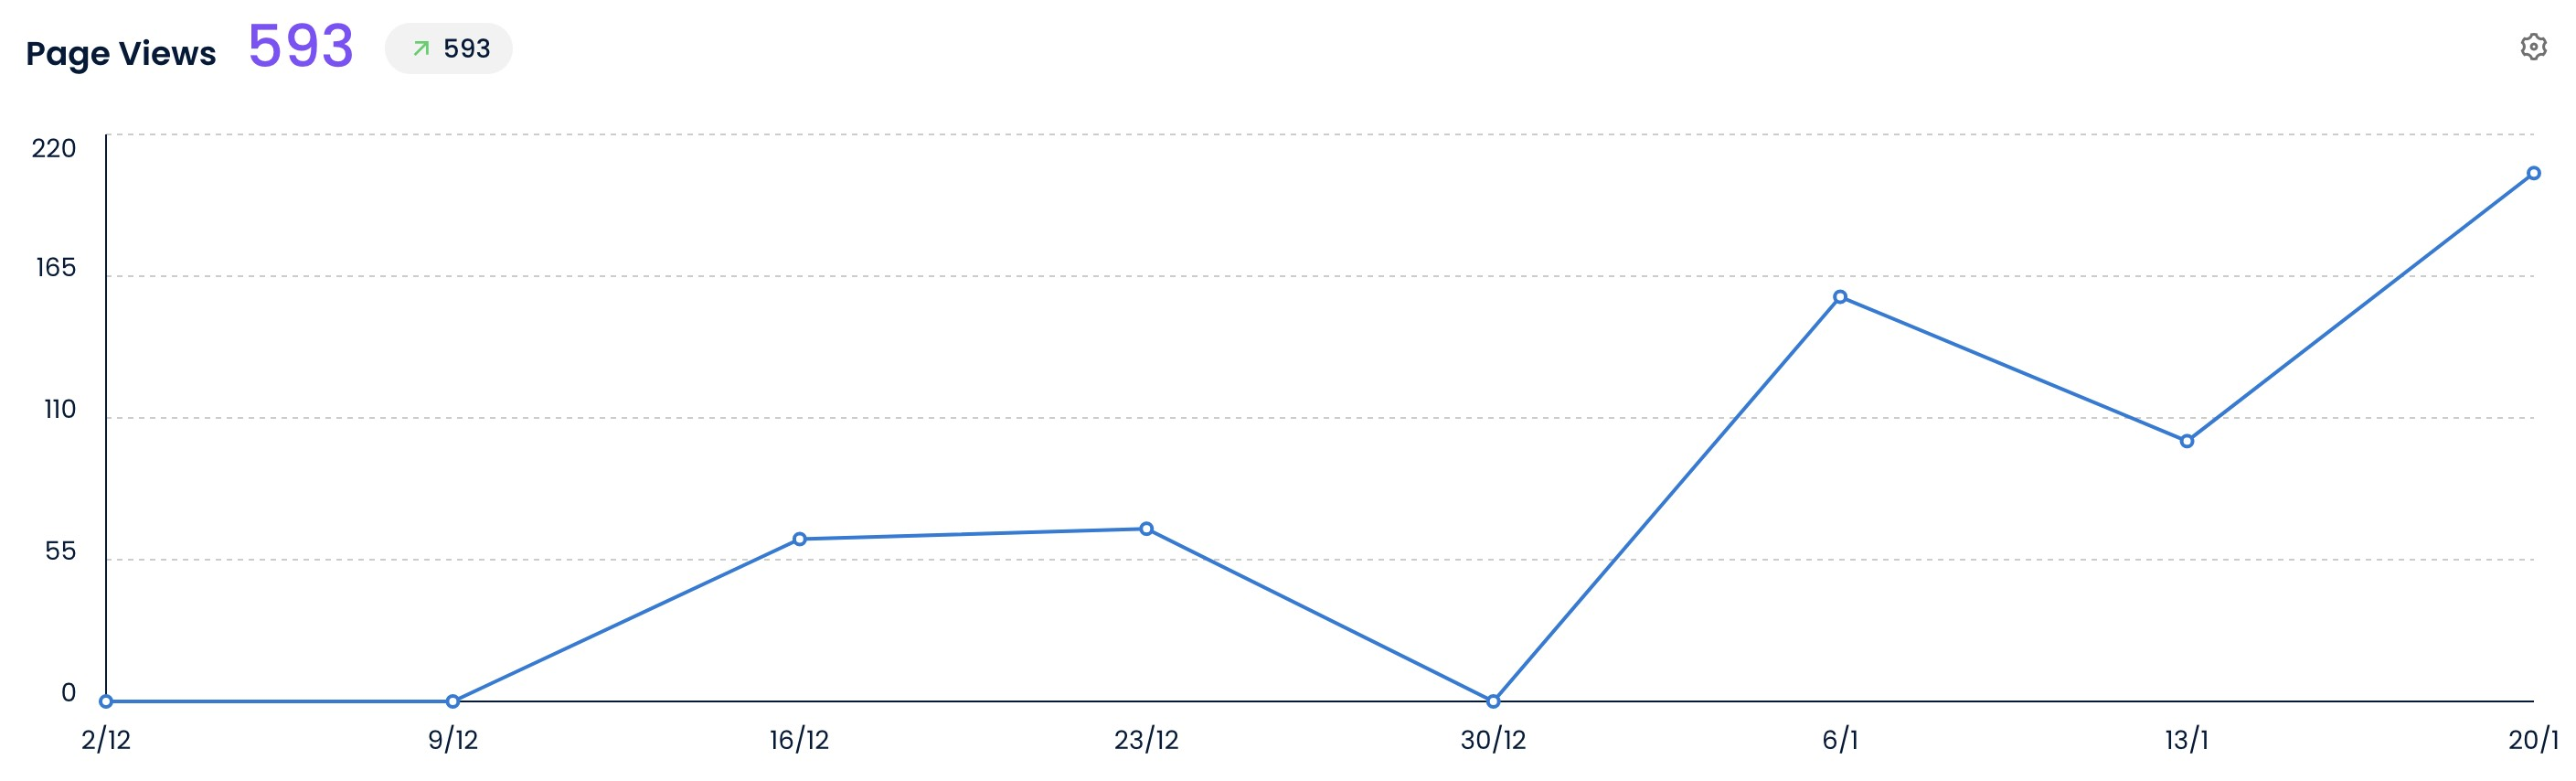
\includegraphics[width=\textwidth]{pics/squeaky_user_curve.jpg}
  \caption{Screenshot: Squeaky.ai page views since December 2022}
  \label{fig:squeaky_users}
\end{figure}

\section{User Testing, Feedback, Beta and Monitoring}

After a first stable deployment was available for stating and production dynamic resources and all basic requirements were met, the user tests for the Beta-phase started.
Four people from our company agreed to use the UI Editor and give verbal feedback. Three of them were already participants of the interviews and they covered all mayor groups of users,
so the feedback represented all different expertise levels.

The reported bugs were written into Jira tickets so the status was properly tracked and release notes could be generated.
Mostly the bugs were edge cases where a file wouldn't open or the changes were not saved properly.


\section{Communication and Documentation}
Communicating with the test users and documenting the technical aspects of the software, the progress and how to use certain features is
another building block towards a good user and developer experience.
\subsection{Asynchronous communication}

For the asynchronous communication, a Microsoft Teams Channel was utilized, a group chat where all invited persons (in case of the internal beta-phase company-wide) can write to each other and create posts. This was used for notifications about new deployments and information about bugs that could affect multiple people.

Even though this adds a bit overhead, it proved easier than having everyone write bug tickets directly, as user often do not know how to describe the problem which leads to unclear descriptions, wrong tags and duplicate tickets.
Instead, a developer with knowledge about the system looked at the reports and created a new ticket if the problem was new, otherwise referenced an existing ticket or forwarded the problem to the responsible team.
Jira tickets were all assigned to the UI builder component as well as specific releases so everyone can see with one click which changes and fixes are contained in which release.

\subsection{Presentation and Beta kickoff}
At the point where the company-wide beta phase started, a presentation meeting was scheduled where I first explained the project,
demonstrated a common work flow and some of the most important features and could directly respond to questions or feedback.
Around 30 employees attended, including quality assurance and customer success managers, covering a wide range of people who possibly will come in touch with the tool.

\subsection{Documentation}
For the feature documentation, Sprylab uses Confluence for internal documentation and Archbee for external documentation that customers can access too.
As we have the common problem of documentation getting postponed indefinitely, I tried to integrate writing documentation directly int o the development flow and only close a ticket if the documentation
was written and reviewed by one additional person. Due to time and personnel shortages, this was unfortunately not always possible and will require more future attention.

